%%%%%%%%%%%%%%%%%%%%%%%%%%%%%%%%%%%%%%%%%
% Structured General Purpose Assignment
% LaTeX Template
%
% This template has been downloaded from:
% http://www.latextemplates.com
%
% Original author:
% Ted Pavlic (http://www.tedpavlic.com)
%
% Note:
% The \lipsum[#] commands throughout this template generate dummy text
% to fill the template out. These commands should all be removed when 
% writing assignment content.
%
%%%%%%%%%%%%%%%%%%%%%%%%%%%%%%%%%%%%%%%%%

\documentclass{article}

\usepackage{fancyhdr} % Required for custom headers
\usepackage{lastpage} % Required to determine the last page for the footer
\usepackage{extramarks} % Required for headers and footers
\usepackage{graphicx} % Required to insert images
\usepackage[utf8]{inputenc}

% Margins
\topmargin=-0.45in
\evensidemargin=0in
\oddsidemargin=0in
\textwidth=6.5in
\textheight=9.0in
\headsep=0.25in 

\linespread{1.1} % Line spacing



\setlength\parindent{0pt} % Removes all indentation from paragraphs

%----------------------------------------------------------------------------------------
%	DOCUMENT STRUCTURE COMMANDS
%	Skip this unless you know what you're doing
%----------------------------------------------------------------------------------------

% Header and footer for when a page split occurs within a problem environment
\newcommand{\enterProblemHeader}[1]{
\nobreak\extramarks{#1}{#1 continued on next page\ldots}\nobreak
\nobreak\extramarks{#1 (continued)}{#1 continued on next page\ldots}\nobreak
}

% Header and footer for when a page split occurs between problem environments
\newcommand{\exitProblemHeader}[1]{
\nobreak\extramarks{#1 (continued)}{#1 continued on next page\ldots}\nobreak
\nobreak\extramarks{#1}{}\nobreak
}

\setcounter{secnumdepth}{0} % Removes default section numbers
\newcounter{homeworkProblemCounter} % Creates a counter to keep track of the number of problems

%----------------------------------------------------------------------------------------
%	NAME AND CLASS SECTION
%----------------------------------------------------------------------------------------

\newcommand{\lessonNumber}[1]{Lezione\ \##1} % Assignment title
\newcommand{\lessonDate}[4]{#1,\ #2\ #3\ #4} % Due date
\newcommand{\lessonCourse}[1]{#1} % Course/class
\newcommand{\lessonTime}[1]{#1} % Class/lecture time
\newcommand{\lessonTeacher}[1]{#1} % Teacher/lecturer
\newcommand{\lessonAuthor}[1]{#1} % Your name
\begin{document}

\section{Progettazione software(9)}

Progettare prima di produrre. Si deve avere un approccio industriale con un metodo ingegneristico, ossia si deve perseguire la \textbf{correttezza per costruzione} e non la correttezza per correzione.

Bisogna cercare di ridurre al minimo lo sforzo della verifica, altrimenti pago un costo doppio. Per cercare di mitigare la verifica uso il principio di riduzione della complessità. La prima cosa che devo fare in un progetto sw è spezzare i problemi in parti più piccole per poterle governare insieme (\textit{divide et impera}).

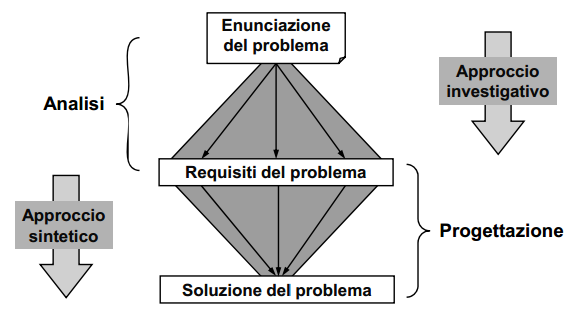
\includegraphics[width=0.5\columnwidth]{img1} % Example image


C'è un'apertura molto grande fatta per frazionamento (\textit{approccio investigativo}) tipico dell'analista. Tutto non è necessariamente esplicito. Il lavoro del progettista è l'esatto opposto, deve riportare a sintesi i requisiti spezzettati e proporre una delle possibili soluzioni al problema, argomentando il valore di quella soluzione. L'analista ha fatto un buon lavoro se i requisiti sono tutti \textbf{tracciabili} e \textbf{verificabili}.\\
Dijkstra afferma che per soddisfare i nostri bisogni:

\begin{itemize}

	\item \textbf{Stabilire le proprietà} di quella cosa in virtù delle quali soddisfo le proprietà attese e i bisogni. Questo è il compito dell'analista.
	\item \textbf{Fare quella cosa} in modo tale che le proprietà attese ci siano. E' quello che fa il progettista.

\end{itemize}

Uno dei compiti che aiuta il progettista è \textbf{fissare un'architettura}, cioè il modo in cui affrontiamo la struttura della soluzione.

Un progettista che lavora strettamente sul progetto fa \textbf{scelte tattiche} sul breve periodo, mentre un architetto ha \textbf{governance}, ha una visione sul lungo periodo. Vogliamo che il progettista si avvicini il più possibile all'architetto. Architettura sw comprende:

\begin{itemize}

	\item Una collezione di software e componenti di sistema, regole e vincoli;
	\item Una collezione di bisogni per gli stakeholders;
	\item Una motivazione per cui la prima collezione soddisfa tutti i bisogni della seconda.
\end{itemize}


Prima di avere componenti, connessioni e vincoli bisogna avere l'idea di come sono le parti, dobbiamo avere un principio costruttivo. Sapere che forma devono avere le parti per ottenere le caratteristiche che mi servono. Esponendo un'interfaccia mostro che cosa offro. Ogni architettura ha uno \textbf{stile} architetturale riconoscibile. Secondo ISO/IEC/IEEE 42010-2011:

\begin{itemize}

	\item L'architettura è un modo per distinguere le parti (\textit{divide});
	\item Quelle parti sono organizzate (\textit{impera});
	\item Per poter avere un'organizzazione di parti bisogna avere delle interfacce che facilitino l'organizzazione;
	\item Paradigma di composizione, il criterio con cui metto insieme queste parti, regole, criteri, vincoli che hanno impatto sulla manutenzione futura.

\end{itemize}

Assunto di aver capito  questo, cerchiamo quali sono le qualità da perseguire in un'architettura:

\begin{itemize}

	\item \textbf{Sufficienza:} soddisfa tutti i requisiti;
	\item \textbf{Comprensibilità:} comprensibile hai portatori d'interesse;
	\item \textbf{Modularità:} fatta di parti facilmente riproducibili e distinte;
	\item \textbf{Robustezza:} sopporta ingressi diversi \textit{(giusti, sbagliati, tanti pochi)};
	\item \textbf{Flessibilità:} permette modifiche a costo contenuto al variare dei requisiti;
	\item \textbf{Riusabilità:} architettura riadattabile a molti altri sistemi, sia nell'insieme che nelle parti;
	\item \textbf{Efficienza:} nel tempo, nello spazio, nelle comunicazioni. Consumare il meno possibile.
	\item \textbf{Affidabilità:} nessun \textit{effetto sorpresa}, riesco a fare ciò che è atteso;
	\item \textbf{Disponibilità:} necessita di poco o nullo tempo di manutenzione \textit{fuori linea};
	\item \textbf{Sicurezza rispetto a intrusioni};
	\item \textbf{Sicurezza rispetto al funzionamento};
	\item \textbf{Semplicità:} ogni parte contiene il necessario e niente di \textit{superfluo}, utilizzo il principio di \textit{Ockham}, elimino tutto quello che è superfluo;
	\item \textbf{Incapsulamento:} (information hiding), nascondo il dettaglio, mostro solo il necessario, in oltre i cresce anche la manutenibilità;
	\item \textbf{Coesione:} le parti che stanno insieme hanno gli stessi obiettivi;
	\item \textbf{Basso accoppiamento:} una modifica ha impatto minimo con gli altri. Le modifiche locali non devono avere effetto sul globale, questo è misurabile ed e composto da due valori, utilità e bisogno.

\end{itemize}

All'inizio della progettazione devo avere sicuramente uno stile architetturale che può essere o \textbf{top-down} (decompone i problemi) o \textbf{bottom-up} (compone le soluzioni). L'approccio normalmente utilizzato è un \textbf{compromesso} fra queste due tecniche, \textbf{meet-in-the-middle}, un approccio intermedio.

Un \textbf{pattern} lo possiamo intendere come soluzioni fattorizzate per problemi ricorrenti.
%slide 27
\end{document}